\chapter{Introducci�n}

Debido a la creciente disponibilidad de las plataformas m�viles y el gran poder de procesamiento con el que cuentan, el n�mero de aplicaciones m�viles ha crecido de manera significativa. Dichas plataformas cuentan con sistemas de adquisici�n de audio, video y una variedad de sensores como por ejemplo aceler�metro y giroscopio, lo que las transforma en sistemas ideales para desarrollar aplicaciones de procesamiento multimedia.\\

Por otro lado, desde hace algunos a\~nos varios museos de distintas partes del mundo han comenzado a considerar este tipo de dispositivos, y otras tantas tecnolog�as, como una alternativa muy interesante para brindar un valor agregado al usuario. Proyecciones de im�genes y videos, recorridos interactivos y aplicaciones de \textit{realidad aumentada} son tan s\'olo algunos de los ejemplos. Sin embargo, esta es un �rea muy reciente y en la que todav�a queda un camino muy largo por recorrer.\\

\begin{figure}[h!]
\centering
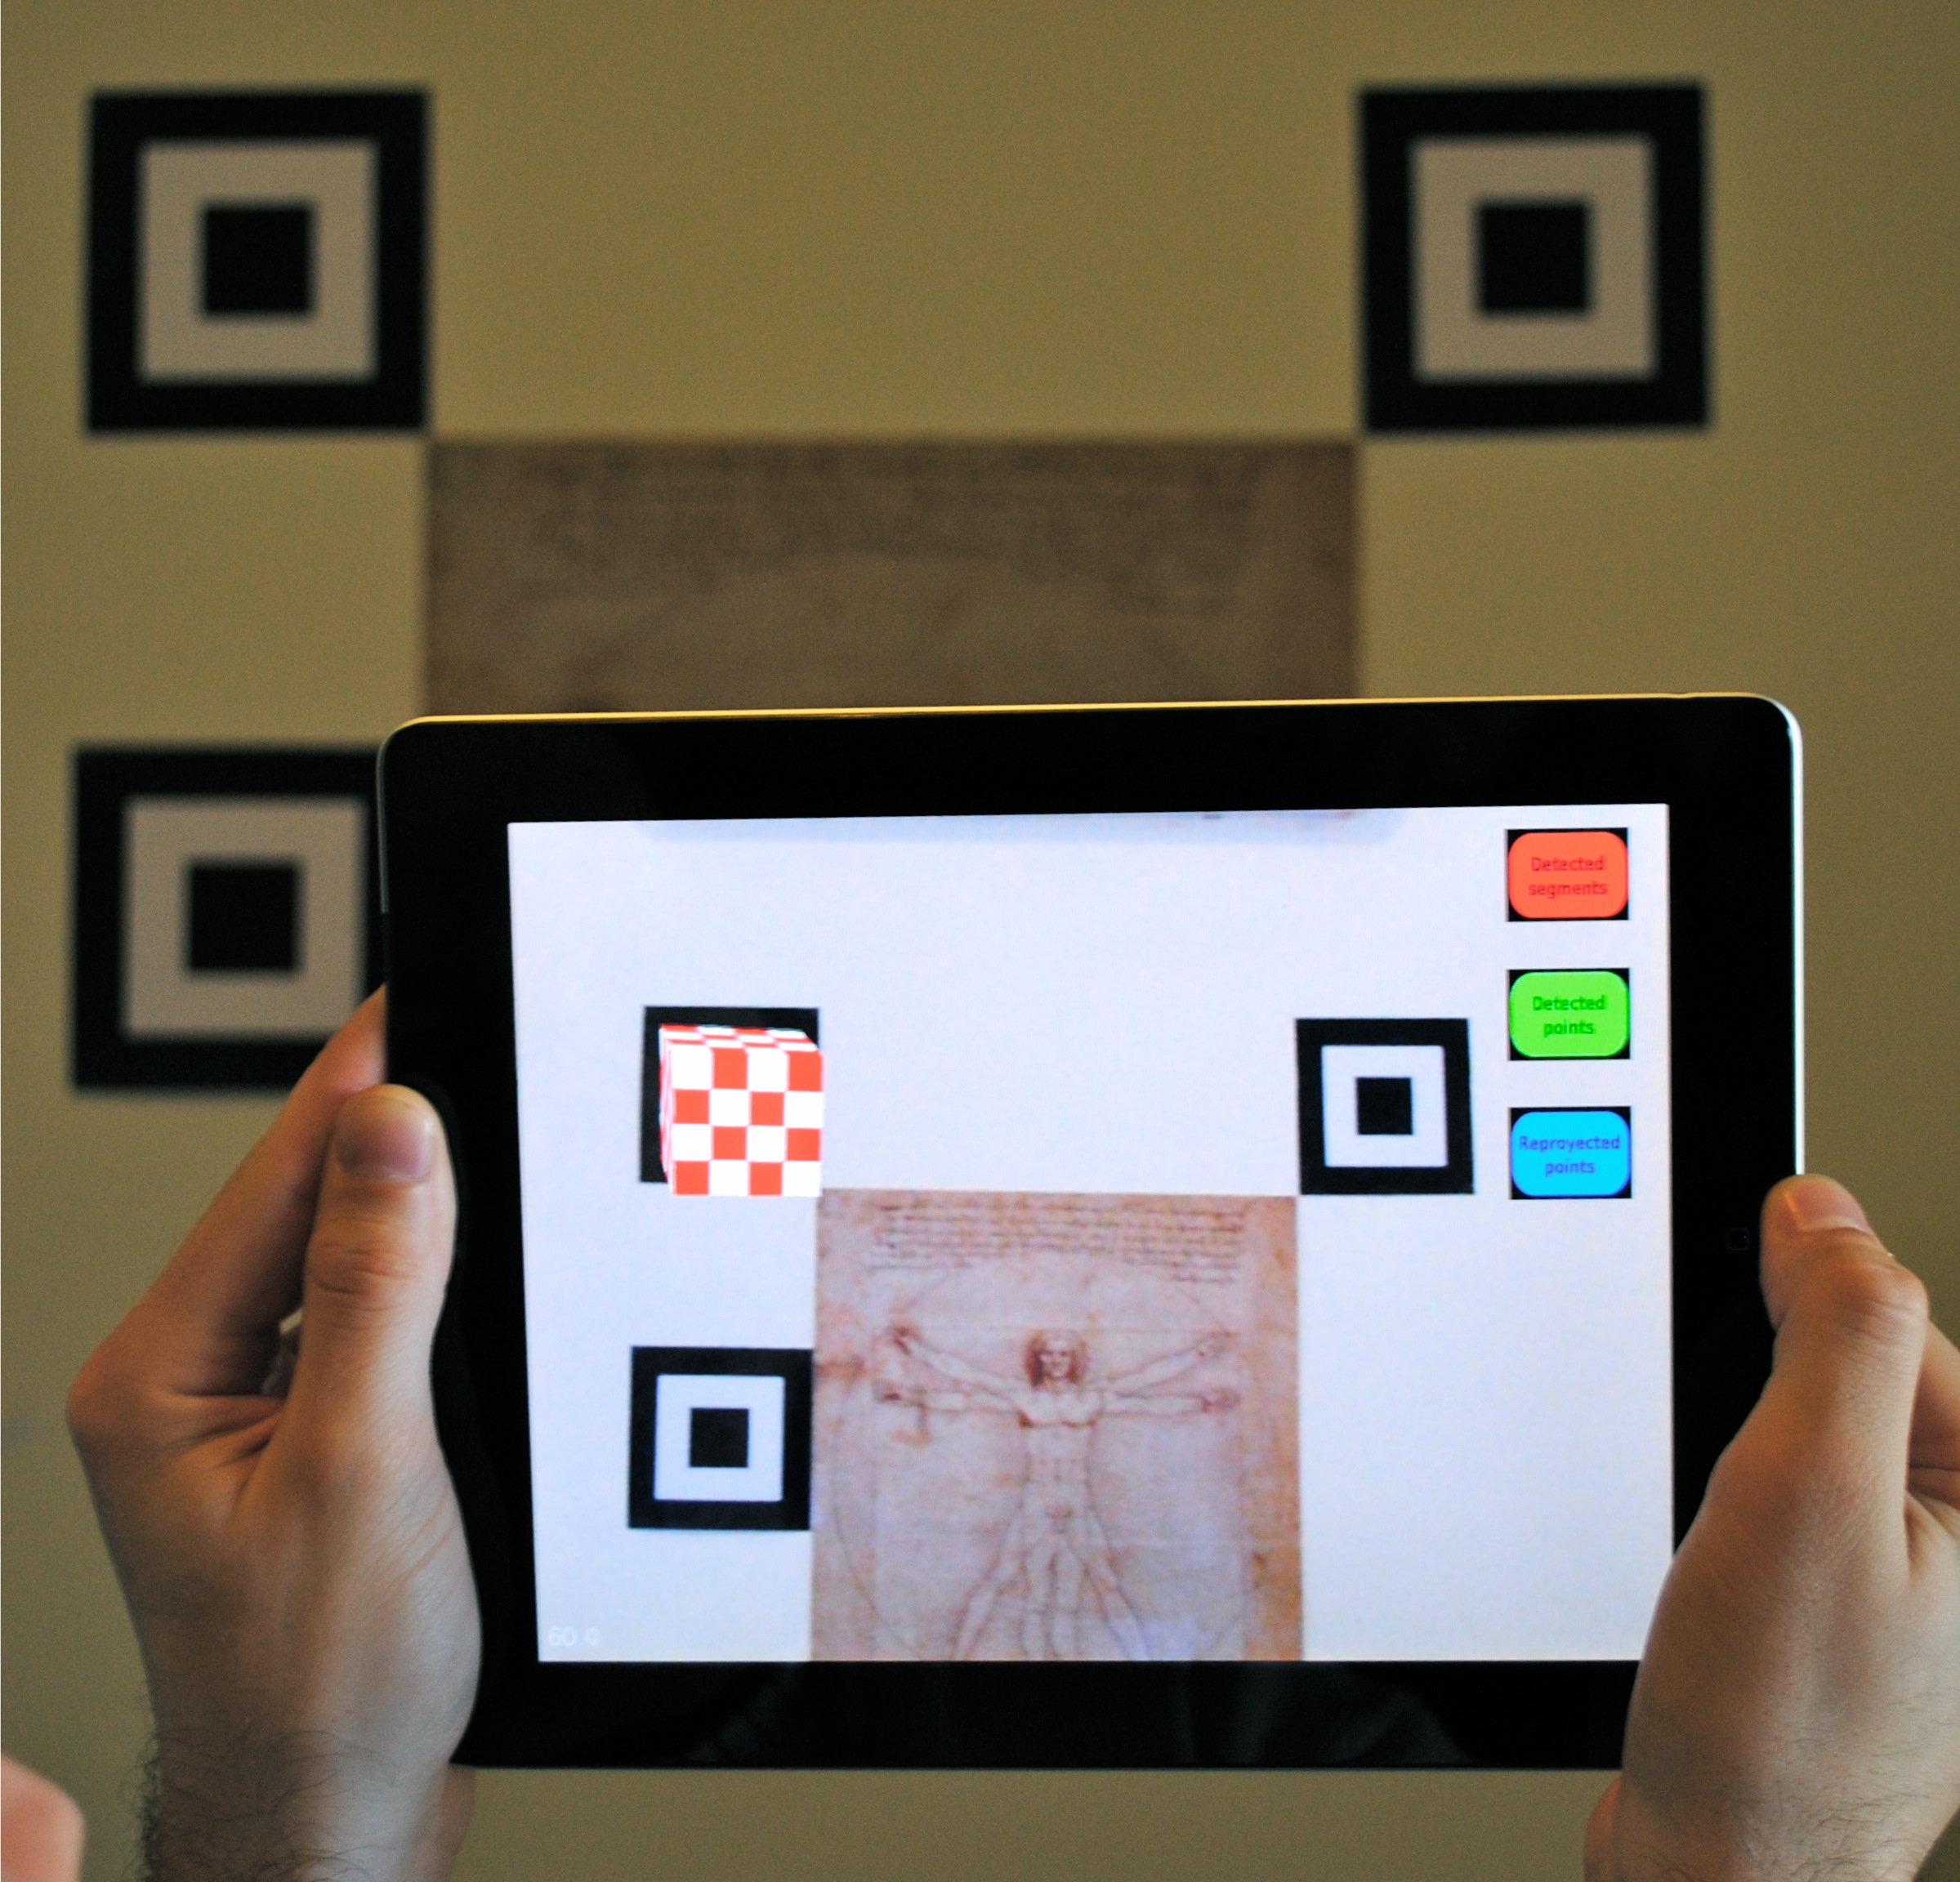
\includegraphics[scale=0.08]{figs_intro/arIntro.png}
\caption{Ejemplo de realidad aumentada.}
\label{fig: arIntro}
\end{figure}

El presente proyecto busca desarrollar sobre ciertos dispositivos m�viles en particular,  un recorrido interactivo para un museo, con realidad aumentada. Se espera de esta manera, contribuir al desarrollo de herramientas que fomenten contenidos educativos y art�sticos, generando as� un marco para poner la tecnolog�a al servicio de la cultura y la sociedad. As� entonces, se estableci� contacto con dos museos de Montevideo, el ``Museo Nacional de Artes Visuales'' (MNAV) y el ``Museo de Arte Precolombino e Ind�gena'' (MAPI). Se espera basar el prototipo final de la aplicaci�n en obras, piezas arqueol�gicas o mapas informativos, pertenecientes a estos dos museos.\\

Probablemente, la realidad aumentada sea el mayor atractivo del proyecto por ser un �rea que se encuentra en pleno desarrollo y que todo el tiempo recibe ideas innovadoras y muy interesantes, lo que la hace por dem�s apasionante. Vale la pena entonces dar una definici�n para la misma:\\

\textit{La realidad aumentada (AR del ingl�s \textit{Augmented Reality}) es un t�rmino que denota la visi�n de un entorno f�sico del mundo real, cuyos elementos se combinan con elementos virtuales generados por computadora, para la creaci�n de una realidad mixta en tiempo real.}\\

Cuando se genera una imagen por medio de realidad aumentada, conviven en ella elementos reales con elementos virtuales. Es b�sicamente un juego de percepciones. En la Figura \ref{fig: arIntro} se puede ver un ejemplo de realidad aumentada, que logra plasmar varios de los conceptos anteriores.\\

A lo largo de la presente documentaci�n se espera dar al lector un panorama de lo que fue el proyecto en su conjunto, esperando que sirva como iniciativa para futuros trabajos vinculados a esta rama de la ingenier�a.